%!TEX root = main.tex

\section{Introduction} % (fold)
\label{sec:introduction}
This experiment involves examining the interactions of neutrons with matter through two experiments using two different detectors. The first detector, a sodium iodide scintillation detector will be used to measure the binding energy of the neutron, and secondly, using a boron-trifluoride counter, measure the moderating properties of water on fast neutrons as a function of radius from a central source.
% section introduction (end)

\section{Detectors} % (fold)
\label{sec:detectors}
This is a section

\subsection{Boron Tri-Flouride Detector} % (fold)
\label{ssub:boron_tri_flouride_detector}
The $\text{BF}_3$ detector contains a boron trifluoride gas at 0.5 to 1 atmospheres which acts as both a target for slow neutron conversion into secondary particles, as well as a proportional gas. A large potential difference is applied across the gas, the cathode held at ground is the outer tube of the detector and the anode, at the high voltage, is a single wire that passes through the centre of the detector, see figure \ref{fig:bf3detector}. When a neutron is incident in the reactor, one of the reaction below takes place.
\begin{align}
	\cf{^{10}_{5}B} + \cf{^{1}_{0}n} &\rightarrow \cf{^{7}_{3}Li} + \cf{^{4}_{2}\alpha} \label{eq:bf31}\\
	\cf{^{10}_{5}B} + \cf{^{1}_{0}n} &\rightarrow \cf{^{7}_{3}Li^*} + \cf{^{4}_{2}\alpha} \label{eq:bf32}
\end{align} 

The products of these two equations differ only by the energy of the lithium which, in some cases, is left in an excited metastable state with a slightly different energy. The relative probabilities of each reaction is 96\% for equation \ref{eq:bf31} and 4\% for equation \ref{eq:bf32}. The resulting ions that are created are attracted to the poles of the detector and so provide a voltage through it. This provides a signal which is sent to the processing computer. It should be noted that this detector cannot give any information of the energy of the neutron since the formation of the ions is independent of energy over a certain level. Instead, this detector is used simply as a counter to obtain a value for the number of neutrons hitting it in a specified time period. 

The electric field close to the wire increases quickly ($E\propto\frac{1}{r^2}$) and so a Townsend avalanche forms near to the wire when a reaction occurs. This involves the electrons being accelerated greatly by the electric field which causes the gas to conduct through the avalanche producing the signal.
\begin{figure}[ht]
	\centering
	\includegraphics[width=0.9\textwidth]{BF3detector.pdf}
	\caption{The $\text{BF}_4$ detector uses a high charge to create a flow of ions to measure the incoming neutron. It cannot measure the energy, but simply gives a count for the number of neutrons incident in the detector.\label{fig:bf3detector}}
\end{figure}

\subsubsection{Wall Effect} % (fold)
\label{ssub:wall_effect}
The BF$_3$ detector shall be used for several purposes later, so it is worth discussing some of the features of the data that is produced by this detector. Figure \ref{fig:walleffect} shows a typical spectrum from the BF$_3$ detector. This shows a main peak, a smaller, higher energy secondary peak and an example of the wall effect.
\begin{figure}[ht]
  \centering
  % \begin{overpic}[width=0.6\columnwidth,grid]{walleffect.pdf}
  \begin{overpic}[width=0.6\columnwidth]{walleffect.pdf}
    \put(20,36){Wall effect}
    \put(20,31){continuum}
    \put(30,30){\vector(-1,-4){4}}
    \put(30,30){\vector(3,-4){10}}
    \put(67,50){$\text{Li}^* + \alpha$}
    \put(80,10){$\text{Li} + \alpha$}
    \put(42,19){$\alpha$}
    \put(30,13){Li}
  \end{overpic}
  \caption{An exemplar spectrum from the BF$_3$ detector showing the wall effect when one of the products from equation \ref{eq:bf31} escapes the detector.\label{fig:walleffect}}
\end{figure}

The two steps in the count number at lower channel numbers is known as the wall effect. These are due to the detector being finite and so there is a chance that one of the products from the reaction escapes from the detector. Due to the relative masses of the particles created, $\alpha$ and Li, the $\alpha$ particle takes most of the energy from the original neutron and so when it is lost from the detector, the recoded energy is lower.

Other features of the spectrum are the abrupt cut-off at the low channel numbers. This is to reduce the background counts that are present in this region from obscuring the rest of the data. 
% subsubsection wall_effect (end)

% sbsubsection boron_tri_flouride_detector (end)

\subsection{Sodium Iodide Detector} % (fold)
\label{ssub:sodium_iodide_detector}
The sodium iodide detector is a scintillation detector that uses a NaI crystal doped with thallium to create scintillation photons when a neutron hits the crystal. The thallium is added as an activator to provide extra available energy levels for the photons in the crystal to occupy. In the pure state, the NaI has a large forbidden band gap between the conduction and valence bands, shown in figure \ref{fig:thaliumactivator}. The activator reduces this gap so that an emitted photon is in the range that the photomultiplier tube is sensitive to, typically visible.
\begin{figure}[ht]
	\centering
	\includegraphics[width=0.9\textwidth]{NaIbands.pdf}
	\caption{The element thallium is added to the pure crystal of sodium iodide to provide extra energy levels for the electrons, which sit inside the forbidden gap of the crystal latice structure. These allow a photon of a useful wavelength to be emitted when electron decays to a lower energy.\label{fig:thaliumactivator}}
\end{figure}

When a gamma photon enters the detector it ionises a molecule of NaI creating excited states in the crystal that then decay via visible photons. The number of photons that are produced is proportional to the energy of the incident photon, as the energy of the gamma ray increases, more scintillation photons are produced. Thus, the energy of the original can be found be counting the number of photons produced. 

These scintillation photons are used to create electrons which are more easily counted. At the photo-cathode, the photons release electrons via the photoelectric effect. The electrons are then passed through the photomultiplier tube which increases the number of photons linearly by accelerating them through a high potential difference so they can knock more electrons out from the dynodes (see figure \ref{fig:naidetctor}). This results in a stream of electrons that can be measured, and which is proportional to the original energy of the photon via the number of scintillation photons, the number of electrons and the multiplication factor of the increase of electrons from the PM tube. Since each of these steps is a linear relationship, a calibration setting can be taken using known results, and a simple linear equation relating the reading taken to the energy of the photon found.
\begin{figure}[ht]
	\centering
	\includegraphics[width=0.9\textwidth]{NaIdetector.pdf}
	\caption{The sodium iodide detector is a commonly used gamma ray detector that uses the relationship between the energy of a photon and the ionisation power that it has to measure its energy via a calibration equation.\label{fig:naidetctor}}
\end{figure}

The detector requires a high voltage which is placed across the dynodes and the anode to accelerate the electrons once they have entered the PM tube. Using this method of acceleration and re-acceleration, the photomultiplier tube is able to increase the number of electrons by a factor of roughly $10^5$ depending on the voltage bias.
\begin{figure}[ht]
	\centering
	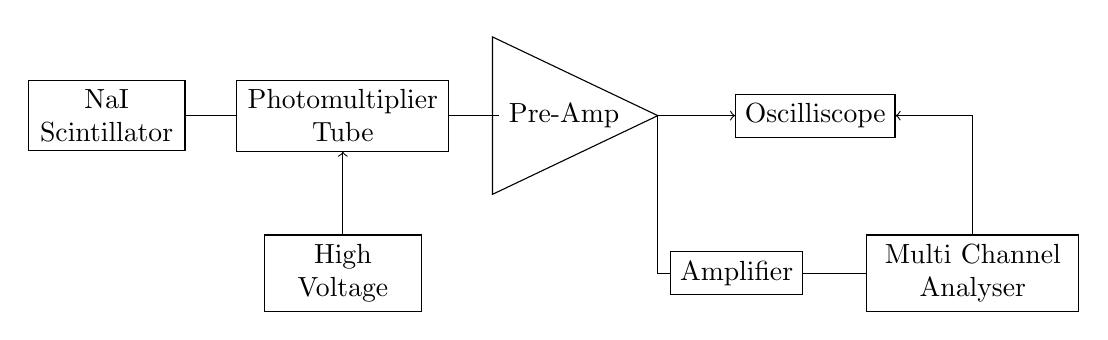
\begin{tikzpicture}
    \node[rectangle, draw, text centered, text width=5em] (1) at (2,0) {NaI Scintillator};
	\node[rectangle, draw, text centered, text width=7em] (2) at (5,0) {Photomultiplier Tube};
	\node[rectangle, draw, text centered, text width=5em] (3) at (5,-2) {High Voltage};
	\node (4) at (7.81,0) {Pre-Amp};
	\node (tri1) at (6.9,1) {	};
	\node (tri2) at (9,0) {	};
	\node (tri3) at (6.9,-1) {};
	\draw (tri1.center) -- (tri2.center) -- (tri3.center) -- cycle;  
	\node[rectangle, draw] (5) at (11,0) {Oscilliscope};
	\node[rectangle, draw] (6) at (10,-2) {Amplifier};
	\node[rectangle, draw, text centered, text width=7em] (7) at (13,-2) {Multi Channel Analyser};
	\draw (1) -- (2);
	\draw[<-] (2) -- (3);
	\draw (2) -- (4);
	\draw[->] (tri2.center) -- (5);
	\draw (6) -| (tri2.center);
	\draw (6) -- (7);
	\draw[->] (7) |- (5);
\end{tikzpicture}
\end{figure}

% subsubsection sodium_iodide_detector (end)
% section detectors (end)
